\section{Software}
Usa el paradigma del productor consumidor, tiene una aplicación que envía y otra que recibe.
\begin{itemize}	
	\item La aplicación de envío ofrece controles para elegir el dispositivo de llegada.
	\item La aplicación receptora utiliza una aplicación web ejecutada en un entorno de Chrome del dispositivo. Se pueden hacer aplicaciones receptoras que aparte de soportar HTML5 tengan más variedad de protocolos de streaming: MPEG-DASH, HTTP Live Streaming, y Microsoft Smooth Streaming Protocol.
\end{itemize}

Chromecast para buscar dispositivos disponibles en una red Wi-Fi usa el protocolo mDNS (multicast Domain Name System), anteriormente usaba el protocolo DIAL (DIscovery And Launch).

Para la visualización de contenidos en la TV se mezclan conceptos DLNA (Digital Living Network Alliance) y Miracast\cite{DLNA-Miracast}.
A la hora de enviar contenido realmente se manda la orden a Chromecast de que reproduzca el contenido elegido directamente desde la nube.
Es la principal diferencia con DLNA, ya que no se reproduce contenido desde un servidor DLNA sino desde Internet.
Para usar solamente DLNA para streaming necesitaríamos aplicaciones de terceros, por ejemplo iMediaShare.
Otra funcionalidad es poder enviar los contenidos de una pestaña del navegador Chrome a la TV en lo que podríamos denominar una conexión Miracast pura y dura, punto a punto.




\begin{figure}[ht] 
	\begin{minipage}[b]{0.55\linewidth}
	Utiliza un sistema operativo de escritorio llamado Chrome OS, siendo el navegador Google Chrome su principal herramienta de uso.  
	Chrome OS se basa en el proyecto de código abierto Chromium OS,5 que, a diferencia de Chrome OS, se puede compilar a partir del código fuente descargado.
	\end{minipage}%%
	\begin{minipage}[b]{0.45\linewidth}
		\centering
		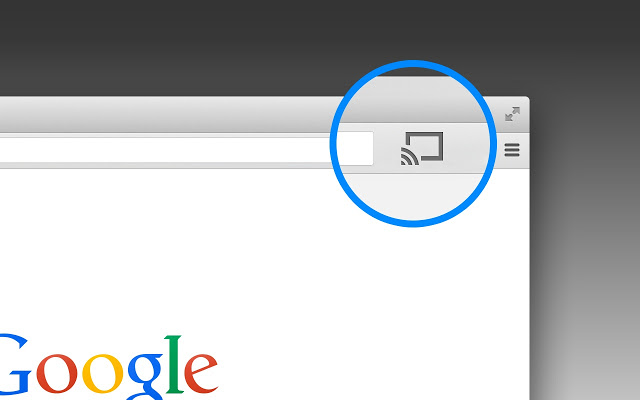
\includegraphics[width=.65\linewidth]{./Imagenes/googlecastbrowser.jpg} 
	\end{minipage} 
\end{figure}







\subsection{Google Cast}
\subsubsection{Google Home}

\subsection{mDNS (multicast Domain Name System)}


\subsection{Miracast}
Miracast es un protocolo multimedia para hacer streaming a un monitor desde un dispositivo local. Para que nuestra smartTV sea capaz de usarlo, necesita soportar Wi-Fi Direct. Wi-Fi Direct es una norma que permite la conexión entre dos dispositivos Wi-Fi sin necesidad de un intermediario.
Los dispositivos que envían y reciben información tienen que estar certificados para Miracast, pero existe un plug para dispositivos no certificados.
Miracast está disponible de manera nativa para dispositivos con versiones de Android 4.2 y Android 6.0.

\vspace{0.1cm}
\begin{figure}[ht]
	\begin{minipage}[b]{0.55\linewidth}
		La conexión está creada vía Wi-Fi Protected Setup (WPS), mecanismos para facilitar la configuración de una red WLAN con seguridad WPA2.
		WPS contempla cuatro configuraciones para el intercambio de credenciales: PIN (Personal Identification Number), PBC (Push Button Configuration), NFC (Near Field Communications) y USB (Universal Serial Bus). La configuración PIN no es recomendable por su debilidad ante ataques de fuerza bruta.
	\end{minipage}%%
	\begin{minipage}[b]{0.45\linewidth}
		\centering
		
\includegraphics[width=.55\linewidth]{./Imagenes/miracast.jpg}
	\end{minipage}
\end{figure}

\

Para la capa de internet usa IPv4; para la de transporte, TCP/UDP, y para la de aplicación, RTSP y RTP, que se encargan de controlar el streaming.

\

A partir de Android 6.0, Google ha dejado de dar soporte nativo a Miracast en favor de su propio Google Cast.
Con Miracast el dispositivo receptor es dependiente de que el dispositivo Android emisor se mantenga activo \cite{Miracast}: si se bloquea también bloqueará la reproducción en el receptor.
Esto implica una mayor carga de trabajo y consumo de batería respecto a Google Cast, que solo se encarga de enviar señales para el control de la reproducción.

\

Existe una alternativa de código abierto a Miracast llamada MiracleCast. El nombre viene por la dificultad de crear una red Wifi-P2P estable (basado en wpa_supplicant).

\

El núcleo de MiracleCast es un demonio llamado miracled \cite{MiracleCast}, que controla links locales, las peticiones de conexión, se encarga de la codificación del protocolo y el parsing.
Su línea de comandos puede ser usada para controlar el demonio, crear nuevas conexiones, modificar parámetros, etc.
Soporta un modo interactivo que muestra las peticiones de conexión y permite al usuario aceptarlas o no.

\

El código fuente se puede encontrar en \href{https://github.com/albfan/miraclecast}{github}.



\subsection{Chrome OS?}